\section{Discussion}


\subsection{Profile plots}


Figure \ref{fig:Profiles} shows the latitude profiles of the different models in differential flux. The flux increases towards the Galactic plane. Left-right assymmetry close to the Galactic center. 


\begin{figure*}[h!]
    \begin{subfigure}{0.5\textwidth}
        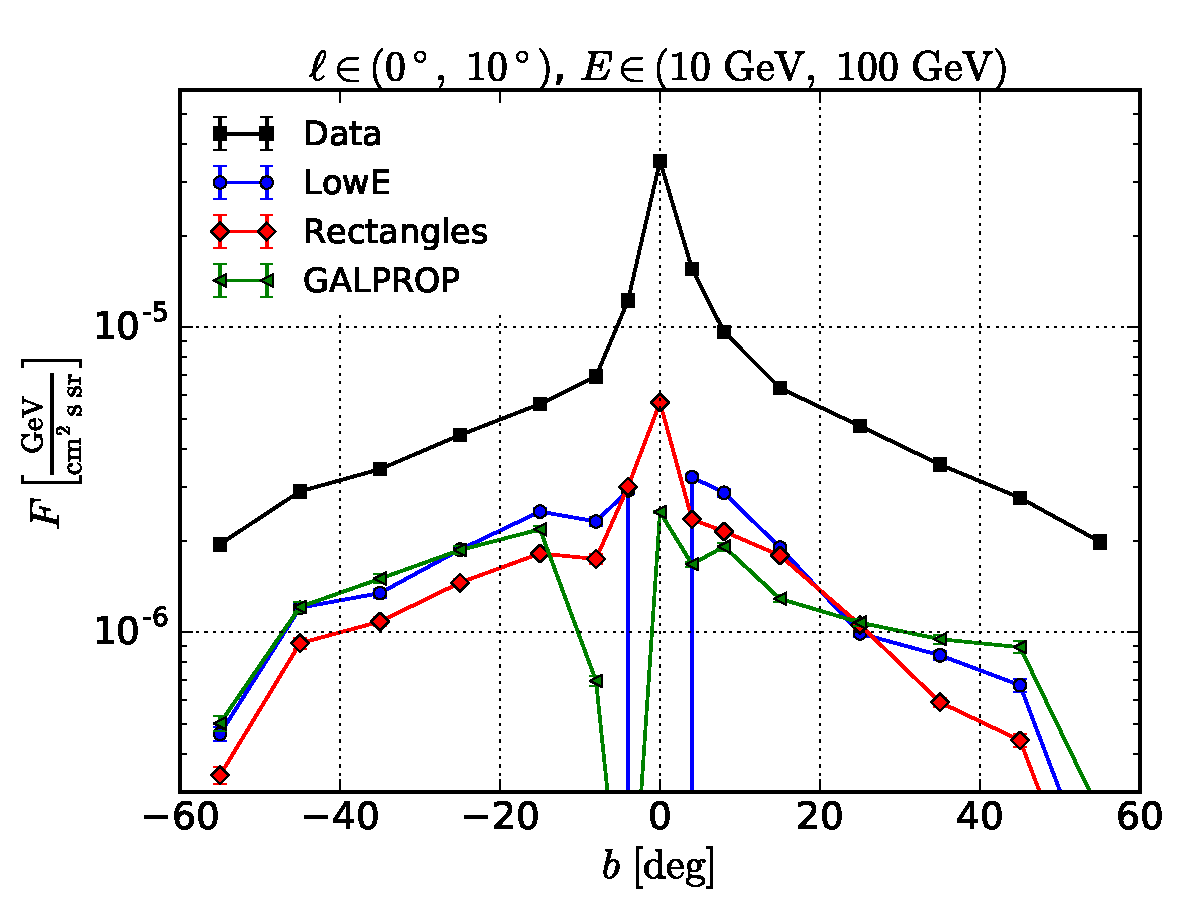
\includegraphics[width=\textwidth]{plots/Profiles_l=1_source_range_1.pdf}
    \end{subfigure} 
    \begin{subfigure}{0.5\textwidth}
        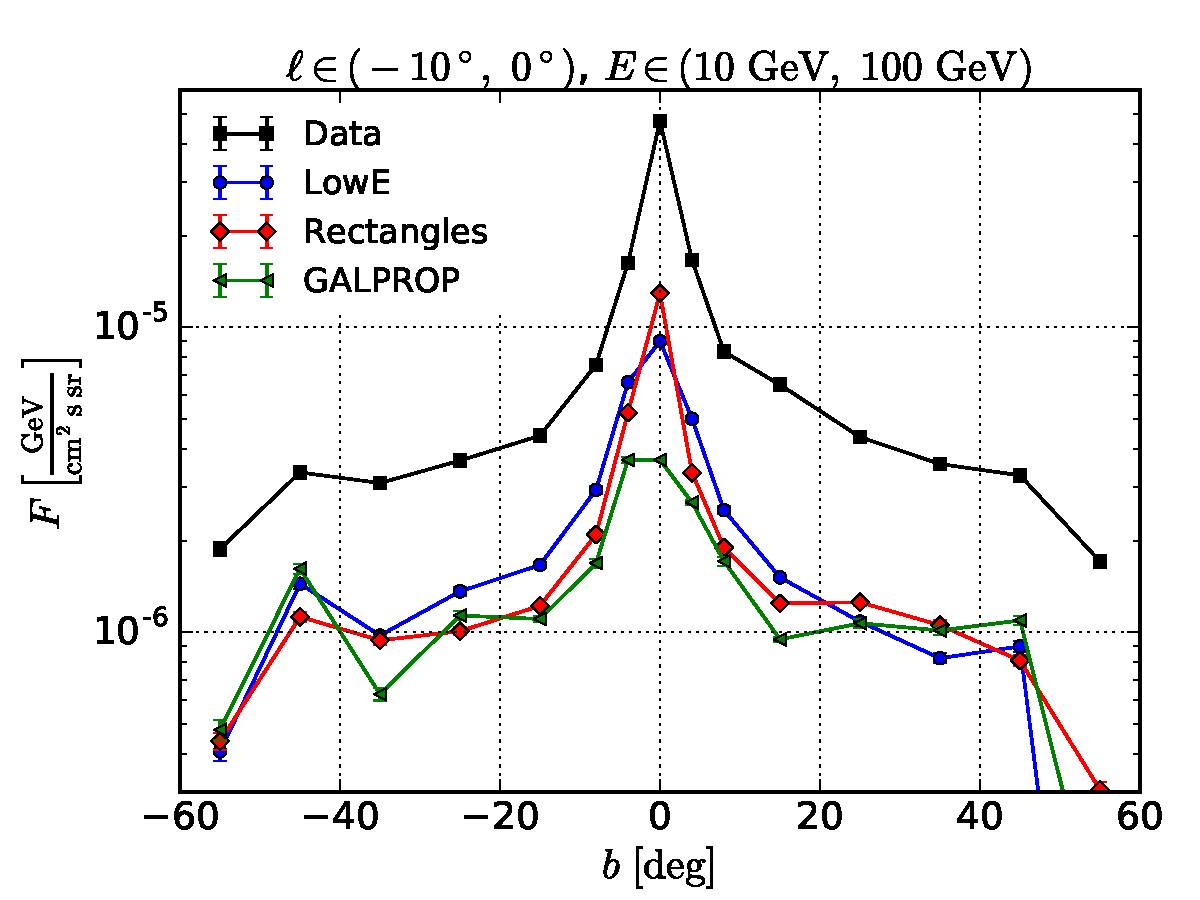
\includegraphics[width=\textwidth]{plots/Profiles_l=0_source_range_1.pdf}
    \end{subfigure}
  	\caption{Latitude profiles of the different models.}
  	\label{fig:Profiles}
\end{figure*}

\subsection{Comparison of the spectra at different latitudes}

Figure \ref{fig:SED_all} shows a comparison of the SED of the raw data (without point sources) and the three different models in a very thin latitude stripe covering the Galactic plane. The grey triangles show the difference in the raw data west minus east. All models give similar results. \\
\\
\begin{figure*}[h!]
    \begin{subfigure}{0.5\textwidth}
        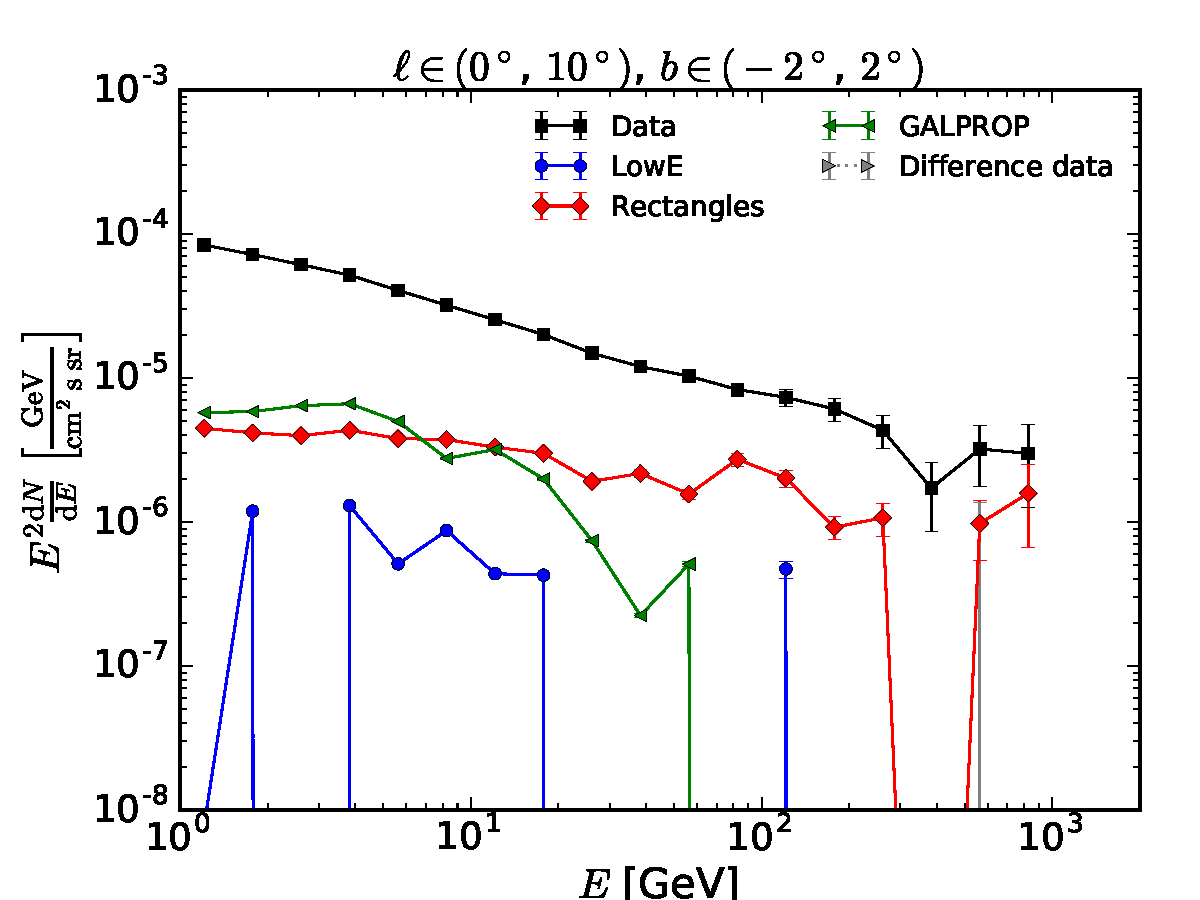
\includegraphics[width=\textwidth]{plots/SED_all_models_source_l=5_b=0.pdf}
    \end{subfigure} 
    \begin{subfigure}{0.5\textwidth}
        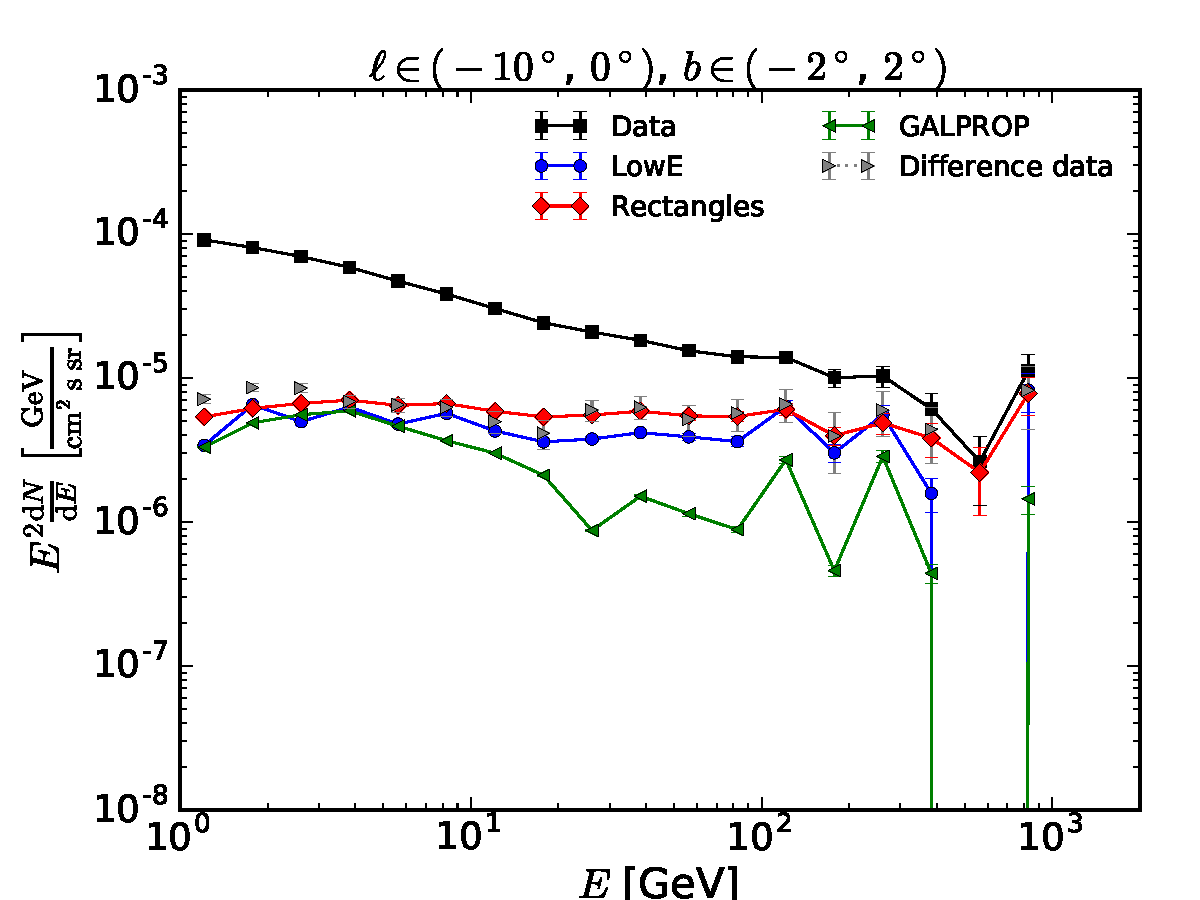
\includegraphics[width=\textwidth]{plots/SED_all_models_source_l=-5_b=0.pdf}
    \end{subfigure}
  	\caption{Comparison of SED of all models.}
  	\label{fig:SED_all}
\end{figure*}
Fit the spectra with a power-law and a cutoff function.
Fit the spectra with IC and pi0 models.

\begin{figure*}[h!]
    \begin{subfigure}{0.5\textwidth}
        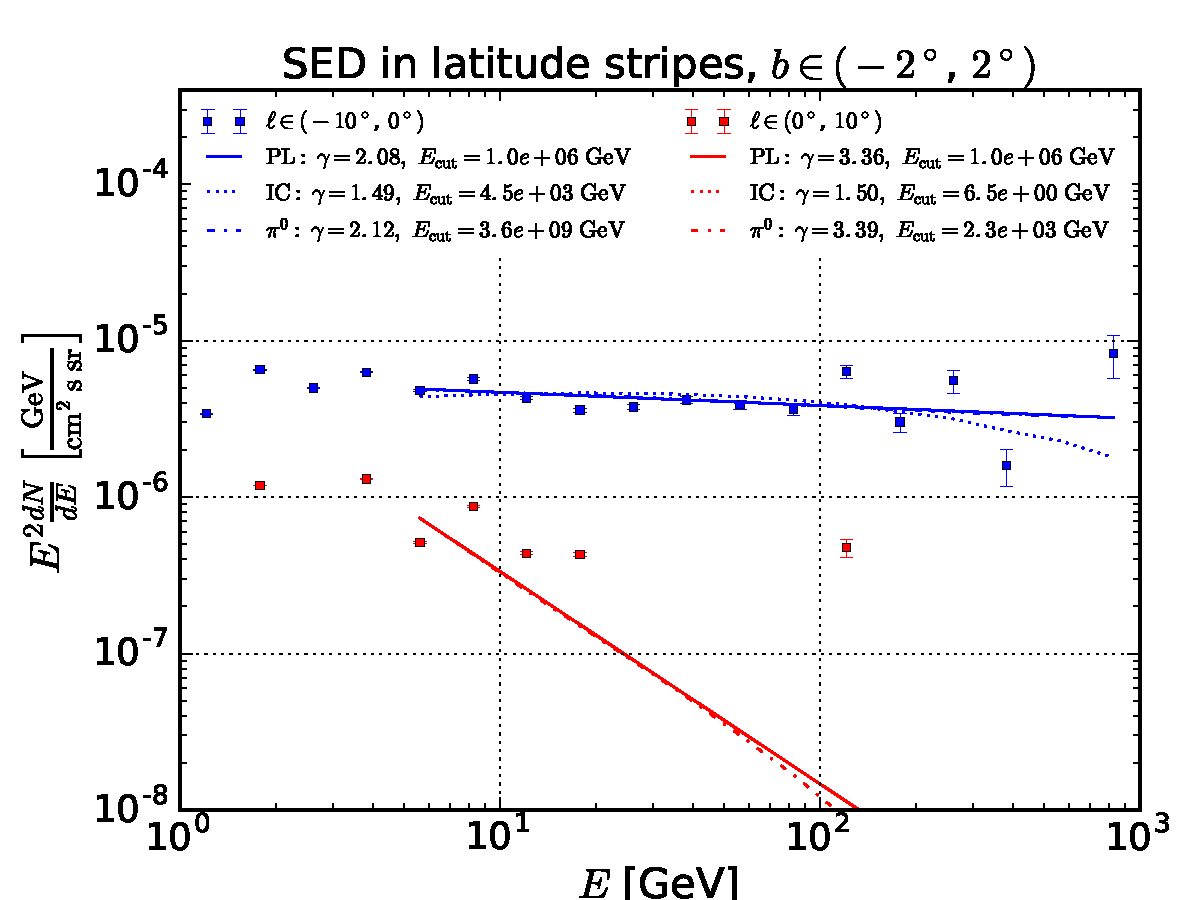
\includegraphics[width=\textwidth]{plots/SED_lowE_source_0cutoff.pdf}
    \end{subfigure} 
    \begin{subfigure}{0.5\textwidth}
        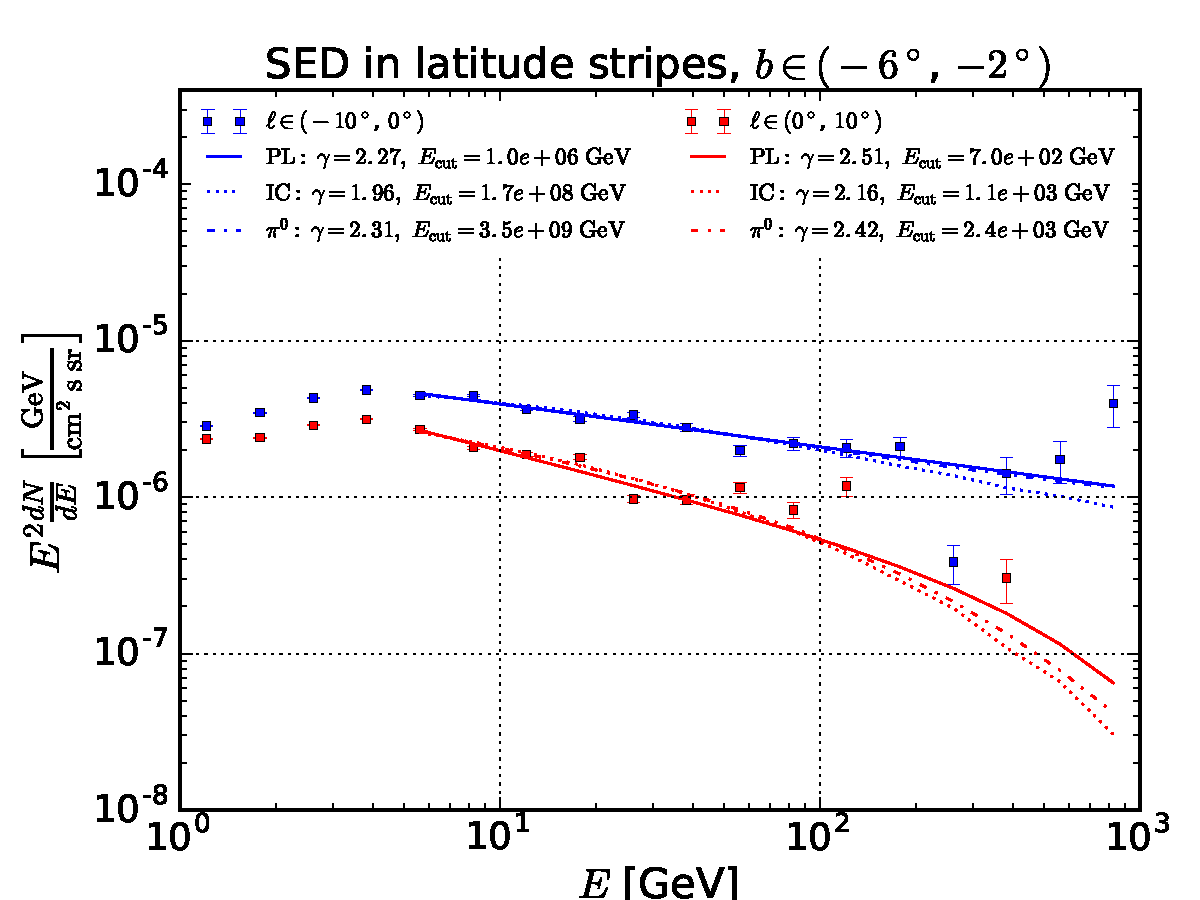
\includegraphics[width=\textwidth]{plots/SED_lowE_source_-4cutoff.pdf}
    \end{subfigure}
  	\caption{SED of low-energy model with powerlaw and particle spectra fits.}
  	\label{fig:SED_with_fits}
\end{figure*}




\subsection{IC model}
\label{sec:IC_model}

IC radiation is produced in scattering processes of relativistic electrons on photons of the ISRF. The spectrum of the IC gamma radiation depends on the density of ISRF photons, the density of electrons and the differential Klein-Nishina cross section $\de \sigma_\IC / \de E_\gamma$, taken from \citep{1970RvMP...42..237B}:
\be
\left(\frac{\de n}{\de E}\right)_{\gamma,\IC} = \int \int \left(\frac{\de n}{\de E}\right)_\ISRF \frac{\de \sigma_\IC}{\de E_\gamma}\left(\frac{\de n}{\de E}\right)_\el \de E_\ISRF \de E_\el.
\label{eq:IC_spectrum}
\ee
The ISRF has three main components: starlight, IR and CMB. The first two components are taken from (???). For the CMB a thermal spectrum of $\SI{2.73}{K}$ is used. We assume that the distribution of electrons follows a powerlaw with a potential cutoff
%\be 
%\left(\frac{\de n}{\de E}\right)_\el = n_\el \left(\frac{E}{\SI{1}{GeV}}\right)^{-\gamma_\el} \cdot \eto^\frac{E}{E_{\cut,\el}},
%\ee
and determine the normalization $n_\el$, spectral index $\gamma_\el$ and cutoff energy $E_\cut$  by fitting the IC spectrum\eqref{eq:IC_spectrum} to the diffuse \Fermi data using Poisson likelihood. Point sources are masked as described in Section \ref{sec:Modeling}. Figure \ref{fig:SED_with_fits} shows the residual spectrum in the low-energy model within the latitude stripes $b \in (-\ang{2}, \ang{2})$ and $b \in (-\ang{6}, -\ang{2})$. The dotted line represents the best-fit IC spectrum.





\subsection{Pion model}
\label{sec:Pion_model}

In collisions of CR protons and the interstellar gas neutral pions are created that decay into gamma-ray photons. The spectrum of the gamma radiation depends on the density of interstellar gas $n_\Hy$, the density and velocity of CR protons and the cross section to produce gamma rays in a proton-nucleus collision:

\be
\left(\frac{\de n}{\de E \de t}\right)_\gamma = \int n_\Hy \frac{\de \sigma_\pr}{\de E_\gamma} v_\pr \left(\frac{\de n}{\de T}\right)_\pr \de T_\pr.
\ee
\dots